% 相反数的定义及函数图象
\begin{frame}{1.2 数轴}
\textbf{规定了原点、正方向和单位长度的直线叫做数轴(number axis). \\
数轴的四要素:} 
\begin{itemize}
    \item \textbf{原点}
    \item \textbf{正方向}
    \item \textbf{单位长度}
    \item \textbf{直线}
\end{itemize}
\vspace{12pt}
\mbox{数轴示例:}
\vspace{12pt}
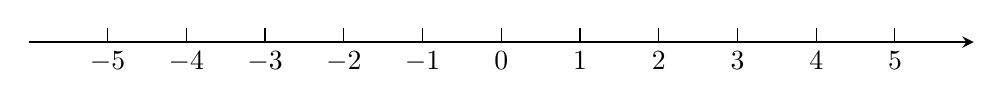
\begin{tikzpicture}
\draw [black, thick, ->, >=stealth] (-6,0) -- (6,0); 
\foreach \x in {-5, ..., 5}
	\draw (\x cm,5pt) -- (\x cm,0pt) node[anchor=north] {$\x$};
\end{tikzpicture}    
\end{frame}

\begin{frame}{1.2 数轴}
\textbf{规定了原点、正方向和单位长度的直线叫做数轴(number axis). \\
数轴的四要素:} 
\begin{itemize}
    \item \textbf{原点}
    \item \textbf{正方向}
    \item \textbf{单位长度}
    \item \textbf{直线}
\end{itemize}
\vspace{12pt}
\mbox{最简数轴:}
\vspace{12pt}
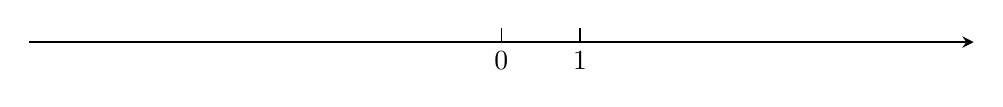
\begin{tikzpicture}
\draw [black, thick, ->, >=stealth] (-6,0) -- (6,0); 
\foreach \x in {0, 1}
 	\draw (\x cm,5pt) -- (\x cm,0pt) node[anchor=north] {$\x$};
\end{tikzpicture} 
\end{frame}